%
% Szakdolgozat minta az Eszterházy Károly Egyetem
% matematika illetve informatika szakos hallgatóinak.
%

\documentclass[
% opciók nélkül: egyoldalas nyomtatás, elektronikus verzió
% twoside, % kétoldalas nyomtatás
% tocnopagenum,% oldalszámozás a tartalomjegyzék után kezdődik
]{thesis-ekf}
\usepackage[T1]{fontenc}
\PassOptionsToPackage{defaults=hu-min}{magyar.ldf}
\usepackage[magyar]{babel}
\usepackage{mathtools,amssymb,amsthm,hyperref,listingsutf8,xcolor,caption,pdfpages}
\usepackage{subcaption}
\lstset{
	inputencoding=utf8,
	language=C,
	basicstyle=\footnotesize,
	breaklines,
	captionpos=b,
	postbreak=\hbox{$\color{red}\hookrightarrow\ $},
	xleftmargin=1cm,
	xrightmargin=1cm,
	backgroundcolor=\color{gray!30},
	frame=tlbr,
	framesep=3pt,
	keywordstyle=\bfseries\color{green!40!black},
	commentstyle=\itshape\color{purple!40!black},
	identifierstyle=\color{blue},
	stringstyle=\color{brown},
	rulecolor=\color{black},
	showstringspaces=false
}

\captionsetup{compatibility=false}
\footnotestyle{rule=fourth}

\newtheorem{tetel}{Tétel}[chapter]
\theoremstyle{definition}
\newtheorem{definicio}[tetel]{Definíció}
\theoremstyle{remark}
\newtheorem{megjegyzes}[tetel]{Megjegyzés}

\begin{document}
\institute{Matematikai és Informatikai Intézet}
\title{Okos otthon hub és irányítóközpont}
\author{Lovász Ákos\\Programtervező informatikus BSc}
\supervisor{Dr. Tajti Tibor\\Egyetemi adjunktus}
\city{Eger}
\date{2021}
\maketitle
\tableofcontents


\chapter*{Bevezetés}
Tanulmányaim folyamán számos technológiával ismerkedtem meg, melyek mindegyike rengeteg
lehetőséget tárt fel előttem, viszont a szakmai gyakorlatom során kiemelkedően megragadta a fantáziámat az Andoid
fejlesztés és a hardverprogramozás összekapcsolása által kialakult rendszerek lehetősége.
\par
Az Android alkalmazások fejlesztése iránt mindig is érdeklődtem, egy-egy kisebb alkalmazást gyakorlásként
már készítettem ezt megelőzően, de komolyabban itt kezdtem vele foglalkozni, megismerkedni a vele járó
sajátosságokkal.
\par
Az ilyen jellegű eszközök kapcsolata és kommunikációja már korai gondolataimban is az okos otthonok felépítésére
emlékeztetett, ezért is gondoltam megfelelő táma választásnak.
\par
A döntést követő kutatás során szembetűnő hátránya volt az okos otthon rendszereknek, hogy a legtöbb ,,márkás''
megoldás elsősorban drága és csak felületes hozzáférést tesznek lehetővé, melyet teljes mértékben a rendszer
gyártója határoz meg. 
\par
Az alternatív, olcsóbb rendszerek bár nyíltabb hozzáállással próbálnak előnyt szerezni,
viszont sokszor erősen a technikai oldalába mélyednek, így egy átlagos felhasználónak bonyolultnak, 
nehezen kezelhetőnek tűnhetnek. Ezen felül gyakran futhatunk olyan problémába, hogy az általunk választott
rendszerben lévő hiányosságokat csak más gyártótól származó eszköz nyújtana megoldást, viszont különböző
gyártók eszközei nagyon ritkán kompatibilisek egymással.
\par
Ezeket az észrevételeket figyelembe véve egyértelműnek tűnt, hogy van lehetőség egy olyan rendszer kivitelezésére,
ami elsősorban olcsóbb, de ugyanakkor nem túlbonyolított, felhasználóbarát marad. Fontos a nyitottság, a bővíthetőség,
és a széleskörű kompatibilitás lehetősége, hogy a felhasználó biztos lehessen abban, hogy a jövőben felmerülő
hiányosságok egyszerűen pótolhatók.

\chapter{A rendszer alapjai}
A rendszer két fő komponensből áll. A kiszolgáló, mely egy Orange PI Zero egykártyás számítógép, amin fut a Node-RED, egy olyan webes felületet biztosító szolgáltatás, mely grafikusan kezelhető komponensek összekapcsolásával teszi lehetővé a renszer működését befolyásolni, és a Mosquitto MQTT bróker, ami lehetővé teszi a Node-RED\cite{nodeRed} és az Androidos alkamazás közötti kommunikációt.

\section{A kiszolgáló hardver}

\begin{figure}[h]
	\begin{subfigure}{0.5\textwidth}
	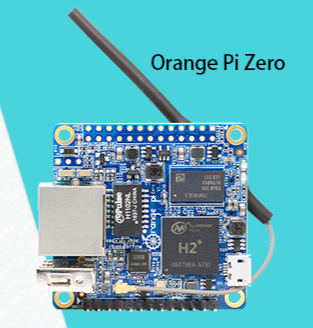
\includegraphics[width=1\textwidth]{images/OPIZero.png}
	\caption{Orange Pi Zero\cite{orange}}
	\label{fig:subim2}
	\end{subfigure}
	\caption{A Node-RED-hez és az MQTT brókerhez használt eszköz}
	\label{fig:image2}
\end{figure}
Az eszköz egy nyílt forráskódu egykártyás számítógép, amin Armbian\cite{armbian} (ARM processzor architektúrára specializált Debian) operációs renszer fut, de lehetőséget nyújt Ubuntu, vagy akár Android operációs rendszer telepítésére is. Ezen fut a Node-RED felület és a Mosquitto MQTT bróker, melyeket a helyi hálózaton bármely eszköz el tud érni, csupán az eszköz IP címét kell ismernie.

\section{Az Android alkalmazás}
Az Androidos alkalmazás célja a felhasználónak hozzáférést nyújtani az összes elérhető eszközhöz, azok állapotát megjeleníteni és felületet biztosítani azok irányítására, állapotuk megváltoztatására. 

A kiszolgálóval való kommunikációt az Eclipse nyílt forráskódú Paho\cite{paho} Androidos kliens oldali MQTT implementációját használatba véve valósítja meg az alkalmazás. 

A kommunikáció két irányú, azaz nem csak az alkalmazás tudja az okos eszközöket irányítani, hanem fogad üzeneteket a kiszolgálótól, így tud naprakész információt prezentálni az eszközök állapotáról a felhasználó számára.

A felület rugalmasságából adódóan az alkamazás nem kizárólag okos otthon kezelésére alkalmas, bármilyen MQTT protokoll alapú rendszeren való kommunikációra képes, viszont miven a fejlesztés során az okos otthonok kezelése volt az elsődleges szempont, így erre a célra használva a legoptimálisabb a felhasználói élmény.

\section{Node-RED}
A Node-RED egy nyílt forráskódú, ,,flow'' alapú programozási eszköz az IBM Emerging Technologies\cite{ibmET} által fejlesztve az OpenJS Foundation\cite{openjs} részeként. Ez egy Node.js alapú fejlesztési eszköz, aminek a felületét egy böngészőn keresztül lehet elérni ahol ,,node''-okat elhelyezve a felületen  egy funkcióhálózatot létrehozva lehet úgymond programozni. Ez a funkcióhálózat egy ,,Deploy'' gomb hatására bekerül a futási környezetbe, így effektíve az eddigi viselkedést felülírva, változtatásainkat elmentve.

\section{MQTT}
Az MQTT (Message Queueing Telemetry Transport)\cite{mqtt} egy OASIS szabványú kommunikációs protokoll, melyet IoT (Internet of Things) eszközök kommunikációjához fejlesztettek ki. A protokoll alapja a ,,Publish/Subscribe'' alapú kommunikáció, azaz egy eszköznek lehetősége van egy adott ,,topic''-ra üzenetet továbbítani, vagy feliratkozni, azaz az adott ,,topic''-on beérkező üzeneteket megkapni. Ezek az üzenetek egy brókeren keresztül érik el céljukat, mivel a bróker tárolja hogy mely eszkör milyen témára iratkozott fel, ez alapján tudja a megfelelő klienseknek továbbítani a megfelelő üzenetet. Mivel az MQTT IoT eszközök kommunikációjához készült, így fejlesztése alatt különös figyelmet fordítottak az erőforrások megspórolásához, ezért ez a protokoll nagyon kevés erőforrást vesz igénybe, szinte bármilyen eszköz használatba tudja venni.

\section{Okos eszközök}
kis eszköz amivel lehet okos eszközt szimulálni
(vagy intergrálásával akár készíteni persze)


\chapter{Hardver}
orangepy, bármi android telefon, okos eszközök (esp32)
\section{Orange Pi Zero}
olyan mint a raspberry csak olcsóbb
\section{Okos eszközök}
esp32
\section{Androidos telefon}
min andr 6.0 kell

\chapter{Szoftver}
nodered, mqtt, android
\section{Node-RED}
kifejtés az aktuális rendszerről
\section{MQTT}
kifejtés az aktuális rendszerről
\section{Android}
kifejtés az aktuális rendszerről
\section{Tesztelés}

\chapter{A renszer működése}
Itt írom le a kész rendszer működését, 
\section{Első indításra felkészítés}
\section{Telefon csatlakoztatása kiszolgálóhoz}
\section{Okos eszközök csatlakoztatása kiszolgálóhoz}
\section{Okos eszközök kezelése az alkalmazásban}

\chapter{Továbbfejlesztési lehetőségek}
user access? felület új eszköztípusok felvételéhez?
cloud service for out of home control

\chapter*{Köszönetnyilvánítás}
\par
Köszönöm a vscode-nak hogy van,
\par
Köszönöm magyarországnak hogy jobban teljesít
\par
Köszönöm a covidnak, hogy átmentem nummatból

\begin{thebibliography}{2}
\bibitem{nodeRed}Node Red forrás,
\\\texttt{\url{https://nodered.org}}

\bibitem{dashboard}Node Red Dashboard forrás,
\\\texttt{\url{https://flows.nodered.org/node/node-red-dashboard}}

\bibitem{orange}Orange Pi forrás,
\\\texttt{\url{http://www.orangepi.org/}}

\bibitem{mqtt}MQTT protokol forrás,
\\\texttt{\url{https://mqtt.org}}

\bibitem{mosquitto}Mosquitto bróker forrás,
\\\texttt{\url{https://mosquitto.org}}

\bibitem{paho}Paho Android MQTT implementáció,
\\\texttt{\url{https://www.eclipse.org/paho/index.php}}

\bibitem{material}Material design forrás
\\\texttt{\url{https://material.io/components/}}

\bibitem{android}Android fejlesztői dokumentáció
\\\texttt{\url{https://developer.android.com/guide}}

\bibitem{armbian}Armbian operációs rendszer
\\\texttt{\url{https://www.armbian.com/}}

\bibitem{iot}IoT based Smart Environment Using Node-Red and MQTT
\\\texttt{Deepthi, B. \& Kolluru, Venkata Ratnam \& Varghese, George \& Narne, Rajendraparasad \& Srimannarayana, Nerella. (2020). IoT based Smart Environment Using Node-Red and MQTT. Journal of Advanced Research in Dynamical and Control Systems. 12. 10.5373/JARDCS/V12I5/20201684.}
\\\texttt{\url{https://www.researchgate.net/publication/342327250_IoT_based_Smart_Environment_Using_Node-Red_and_MQTT}}
	
\bibitem{android refrences book}Android\texttrademark Notes for Professionals book
\\\texttt{\url{https://books.goalkicker.com/AndroidBook/}}

\bibitem{ibmET}IMB Emerging Technologies
\\\texttt{\url{https://emerging-technology.co.uk/}}

\bibitem{openjs}OpenJS Foundation
\\\texttt{\url{https://openjsf.org/}}

\end{thebibliography}
%\includepdf{nyilatkozat.pdf}
\end{document}